\documentclass[10.5pt]{article}
\usepackage{amssymb} 
\usepackage{color}
\usepackage{graphicx}
\usepackage[a4paper,bindingoffset=0.2in,
            left=3.35cm,right=2.12cm,top=3.75cm,bottom=2.88cm,
            footskip=.25in]{geometry}
\usepackage[T1]{fontenc}
\usepackage{hyperref}
\hypersetup{
    colorlinks=true,
    linkcolor=black,
    citecolor=black,
    filecolor=black,
    urlcolor=black
}
\usepackage{todonotes}
\usepackage{tabularx}
\usepackage{minted}
\usepackage{etoolbox}
\usepackage{amsmath}
\usepackage{amsfonts}
\usepackage{siunitx}
\usepackage{booktabs}
\usepackage{caption}
\usepackage{subcaption}
\usepackage{url}

\makeatletter
\pretocmd{\section}{\clearpage}{}{}
\makeatother

\begin{document}

%%%%%%%%%%% TITLE PAGE
\begin{titlepage}
\begin{figure}[t]
    \centering
    
\includegraphics[width=0.5\textwidth]{HSLU2022logo.svg.png}
\end{figure}

\begin{center}
    \textsc{\LARGE{Hochschule Luzern\\}}
    \textsc{\LARGE{Computer Science Department\\}} 
    \vspace{40mm}
    \fontsize{10mm}{7mm}\selectfont 
    \textup{DSPRO2: Optimizing Machine Learning Models for Commonsense Question Answering}\\
\end{center}

\vspace{25mm}

\begin{minipage}[t]{0.47\textwidth}
    \textnormal{\large{\bf Lecturers / Coaches\\}} 
    {\large Dr. Umberto Michelucci\\ 
    Dr. Seraina Glaus\\
    Dr. Curdin Derungs\\
    Fabian Widmer}
\end{minipage}\hfill\begin{minipage}[t]{0.47\textwidth}\raggedleft
    \textnormal{\large{\bf Candidates\\}}
    {\large Aditi Sharma\\
    Luke Kronenberg\\
    Daniel Betschart}
\end{minipage}

\vspace{20mm}

\centering{\large{Year 2025}} 

\end{titlepage}
\newpage
\tableofcontents
\newpage


\begin{abstract}
Commonsense question answering (CQA) remains a significant frontier in artificial intelligence, requiring models to perform human-like reasoning on everyday knowledge. This project, DSPRO2, undertakes a comprehensive exploration and optimization of various machine learning architectures for the CommonsenseQA benchmark dataset. We systematically evaluated three distinct categories of models: (1) traditional NLP approaches using FastText embeddings with feedforward and recurrent neural network (RNN/LSTM) classifiers; (2) transformer-based models, specifically ALBERT (albert-base-v2), both by fine-tuning pre-trained weights and training from random initialization; and (3) prompting techniques with the Large Language Models (LLM) google/flan-t5-large and deepseek-ai/DeepSeek-R1, including zero-shot, few-shot, zero-shot Chain-of-Thought (CoT), and Retrieval Augmented Generation (RAG) with live web search. Beyond these, our exploration extended to more advanced hybrid architectures. We developed a Hybrid RoBERTa-BiLSTM-ODE Model which combines RoBERTa, BiLSTM, and an ODE-based diffusion component, enhanced by ConceptNet knowledge for sequential dependency capture and feature refinement, achieving a best validation accuracy of approximately 37.50\%. Furthermore, we investigated novel neuro-symbolic approaches, including a Basic Neuro-Symbolic QA Model that integrates neural encoders (RoBERTa, LSTM) with symbolic knowledge graphs from ConceptNet processed by Graph Neural Networks (GNNs), yielding a best validation accuracy of approximately 42.67\%. This was further advanced in the Advanced Gated Neuro-Symbolic QA Model, which employs sophisticated cross-attention and gated fusion mechanisms to dynamically combine neural and symbolic representations, achieving a best validation accuracy of 59.33\%. Our findings reveal a clear performance hierarchy: traditional models achieved accuracies near random chance ($\approx$20\%), underscoring their limitations. Fine-tuned ALBERT showed substantial improvement (54.38\% accuracy), while ALBERT trained from scratch performed poorly, highlighting the critical impact of pre-training. The Flan-T5-large model demonstrated the highest efficacy, with zero-shot and few-shot prompting achieving impressive accuracies of 85.83\% and 85.09\% respectively. RAG also showed promise (78.00\% on a subset), while CoT prompting resulted in a performance decrease (62.98\%). The hybrid and neuro-symbolic models provided insights into architectural complexities and knowledge integration strategies for improving commonsense reasoning, exploring a diverse spectrum of deep learning and symbolic methodologies beyond conventional fine-tuning. This study emphasizes the pivotal role of large-scale pre-training and advanced architectures (Transformers, LLMs) in tackling commonsense reasoning, and provides insights into the varying effectiveness of different prompting strategies.
\end{abstract}

\newpage

%%%%%%%%%%% MAIN CONTENT

\section{Introduction}
This report details the project "DSPRO2", which focuses on the optimization of machine learning models for the task of commonsense question answering. The primary objective, as outlined in the project's scope, is to explore various architectural approaches and methodologies to enhance model performance on questions that require a significant degree of commonsense reasoning. Commonsense question answering (CQA) is a challenging subfield of Natural Language Processing (NLP) that aims to develop systems capable of answering questions that humans typically find trivial, yet require a foundational understanding of the world.

The project utilizes the CommonsenseQA dataset, a widely recognized benchmark available on Hugging Face. This dataset consists of multiple-choice questions, where each question is accompanied by five possible answer choices, and the model's task is to select the most plausible answer. Successfully tackling this dataset necessitates models that can go beyond simple pattern matching and engage in deeper reasoning processes.

Throughout this project, several distinct architectural paradigms were implemented and evaluated. These include:
\begin{enumerate}
    \item Traditional NLP approaches leveraging pre-trained word embeddings (FastText) in conjunction with:
        \begin{itemize}
            \item A 2-layer feedforward neural network classifier.
            \item A Recurrent Neural Network (RNN) architecture (LSTM/GRU) followed by a classifier.
        \end{itemize}
    \item Transformer-based models, specifically focusing on the ALBERT (`albert-base-v2`) architecture. Experiments were conducted by:
        \begin{itemize}
            \item Fine-tuning the pre-trained ALBERT model.
            \item Training an ALBERT model from random initialization to assess the impact of pre-training.
        \end{itemize}
    \item Prompting techniques with Large Language Models (LLMs), using `google/flan-t5-large` and `deepseek-ai/DeepSeek-R1` to explore:
        \begin{itemize}
            \item Zero-shot prompting.
            \item Few-shot prompting.
            \item Zero-shot Chain-of-Thought (CoT) prompting.
            \item A Retrieval Augmented Generation (RAG) pipeline incorporating live web search via SerpAPI.
        \end{itemize}
    \item Advanced hybrid and neuro-symbolic architectures, pushing the boundaries of knowledge integration and reasoning:
        \begin{itemize}
            \item A Hybrid RoBERTa-BiLSTM-ODE Model.
            \item A Basic Neuro-Symbolic QA Model.
            \item An Advanced Gated Neuro-Symbolic QA Model.
        \end{itemize}
\end{enumerate}

The central research question guiding this project can be formulated as: \textbf{How do different neural network architectures, ranging from traditional word embedding-based models to advanced transformer and large language models, compare in performance and efficiency for commonsense question answering, and what are the key factors influencing their optimization?}

This report will detail the dataset, preprocessing steps, methodologies employed for each architectural approach, experimental setup including hyperparameter tuning and model validation strategies, and a comprehensive analysis of the results obtained. All experiments and metrics were tracked using Weights \& Biases (W\&B) to ensure reproducibility and facilitate comparison. The findings aim to provide insights into effective strategies for optimizing models for commonsense reasoning tasks.

\section{Related Works (Literature Review)}
Commonsense question answering (CQA) represents a significant challenge in artificial intelligence, requiring models to possess a level of understanding akin to human intuition. This literature review explores key advancements and methodologies relevant to this project, spanning word embeddings, recurrent and transformer architectures, fine-tuning strategies, and prompting techniques for large language models.

\subsection{Commonsense Question Answering and Datasets}
The CommonsenseQA dataset (Talmor et al., 2019) is a prominent benchmark specifically designed to test commonsense reasoning. It presents questions that require knowledge about everyday situations, object properties, and social interactions, making it distinct from factoid-based QA datasets. Other similar datasets, such as PIQA (Physical Interaction QA) (Bisk et al., 2020) and Social IQA (Sap et al., 2019), also aim to evaluate different facets of commonsense knowledge. The primary challenge in CQA lies in equipping models with the implicit knowledge humans use effortlessly. Early approaches often struggled due to the lack of explicit commonsense knowledge bases integrated into neural models. Research by Liu et al. (2020) on "Commonsense Reasoning for Goal-Directed Dialogue" further highlighted the need for models to incorporate diverse forms of commonsense for practical applications.

\subsection{Word Embeddings for NLP}
Word embeddings revolutionized NLP by representing words as dense vectors in a continuous space, capturing semantic relationships. FastText (Bojanowski et al., 2017), used in this project's initial experiments, enhances traditional word vector models like Word2Vec (Mikolov et al., 2013a) by incorporating subword information. This allows FastText to generate embeddings for out-of-vocabulary words and often better capture morphological nuances. While effective for many tasks, averaging word embeddings for sentences or longer texts, as done in one of our approaches, can lead to a loss of sequential information and nuanced meaning, which is often critical for complex reasoning tasks (Mikolov et al., 2013b).

\subsection{Recurrent Neural Networks (RNNs) in Question Answering}
RNNs, particularly LSTMs (Hochreiter \& Schmidhuber, 1997) and GRUs (Cho et al., 2014), were a significant step forward in processing sequential data like text. Their ability to maintain a hidden state allows them to capture dependencies across tokens in a sequence. In question answering, RNNs have been used to encode both the question and the answer choices (or context passages) into fixed-size vectors, which are then used for classification or similarity computation (Wang \& Jiang, 2016). For instance, Hermann et al. (2015) demonstrated the use of attentive LSTMs for reading comprehension. However, RNNs can struggle with very long-range dependencies and are computationally intensive to train compared to newer architectures.

\subsection{Transformer Models for Question Answering}
The advent of the Transformer architecture (Vaswani et al., 2017), with its self-attention mechanism, marked a paradigm shift in NLP. Models like BERT (Devlin et al., 2019) and its variants demonstrated state-of-the-art performance on numerous benchmarks, including QA. ALBERT (A Lite BERT for Self-supervised Learning of Language Representations) (Lan et al., 2020), used in this project, introduced parameter-reduction techniques to lower memory consumption and increase training speed compared to BERT, while often maintaining or improving performance. ALBERT, like BERT, is pre-trained on massive text corpora using self-supervised objectives (like Masked Language Modeling and Sentence Order Prediction), enabling it to learn rich contextual representations. For multiple-choice QA, models like `AlbertForMultipleChoice` are specifically designed to process a question along with several candidate answers and predict the most plausible one. Further advancements like RoBERTa (Liu et al., 2019) showed that robustly optimizing the pre-training process of BERT-like models can lead to significant performance gains.

\subsection{Fine-tuning Strategies for Pre-trained Language Models}
Fine-tuning pre-trained language models (PLMs) on downstream tasks is a dominant paradigm in modern NLP (Howard \& Ruder, 2018). The process typically involves adding one or more task-specific layers on top of the PLM and then training the entire model (or a subset of its layers) on task-specific labeled data. Effective fine-tuning often requires careful hyperparameter selection (e.g., learning rate, batch size, number of epochs) to avoid issues like catastrophic forgetting or overfitting to the smaller downstream dataset. Strategies such as using a smaller learning rate for the PLM layers compared to the task-specific layers, and employing gradual unfreezing, have been explored to optimize this process (Sun et al., 2019). Raffel et al. (2020) in their T5 paper also explored a unified text-to-text framework where various NLP tasks, including QA, are cast as text generation problems, relying on effective fine-tuning.

\subsection{Prompting Techniques for Large Language Models (LLMs)}
Large Language Models (LLMs) like GPT-3 (Brown et al., 2020) and Flan-T5 (Chung et al., 2022) have shown remarkable capabilities in performing tasks with minimal or no task-specific training, through prompting.
\begin{itemize}
    \item \textbf{Zero-shot prompting} involves directly querying the LLM with the task instance without providing any examples.
    \item \textbf{Few-shot prompting} provides the LLM with a few examples of the task (input-output pairs) in the prompt before the actual query, enabling in-context learning.
    \item \textbf{Chain-of-Thought (CoT) prompting} (Wei et al., 2022) encourages LLMs to generate intermediate reasoning steps before arriving at a final answer, which has been shown to improve performance on complex reasoning tasks. Kojima et al. (2022) further showed that even a simple prompt like "Let's think step by step" can elicit reasoning in zero-shot settings.
    \item \textbf{Retrieval Augmented Generation (RAG)} (Lewis et al., 2020) combines PLMs with non-parametric memory, typically a retriever that fetches relevant documents or text snippets from a large corpus (like the web in this project via SerpAPI) to provide context for the LLM's generation process. This helps ground LLMs in factual information and can reduce hallucination.
\end{itemize}
The effectiveness of these techniques often depends on the LLM's scale, the nature of the task, and the quality of the prompts and retrieved context.

\subsection{Hybrid and ODE-based Architectures in NLP}
Recent advancements in deep learning have led to the exploration of hybrid architectures that combine the strengths of different neural paradigms to address complex NLP challenges. For instance, while Transformer models excel at capturing long-range dependencies through self-attention, Recurrent Neural Networks (RNNs) like LSTMs remain effective for sequential modeling and capturing local context. Combining these, as seen in the Hybrid RoBERTa-BiLSTM-ODE Model developed in this project, allows for leveraging the contextual understanding of pre-trained Transformers (Liu et al., 2019 for RoBERTa) with the sequence-processing capabilities of RNNs.
A particularly novel direction involves integrating Ordinary Differential Equations (ODEs) into neural networks, leading to Neural ODEs (Chen et al., 2018). In NLP, Neural ODEs have been explored for tasks requiring continuous dynamics, such as modeling temporal sequences or refining representations over continuous transformations (e.g., in flow-based models). Their application in diffusion models, which iteratively refine data towards a target distribution, offers a unique mechanism for improving feature representations in complex tasks like question answering.

\subsection{Neuro-Symbolic Approaches for Commonsense Reasoning}
Purely neural Large Language Models (LLMs) often struggle with explicit reasoning and interpretability (Marcus, 2020; Bender et al., 2021). This has led to neuro-symbolic AI, combining neural networks for pattern recognition with symbolic methods for knowledge and logical inference (Garcez et al., 2019). A key aspect is integrating external structured knowledge, like commonsense knowledge graphs such as ConceptNet (Speer et al., 2017), from which models extract relevant facts. Graph Neural Networks (GNNs), including GCNs (Kipf \& Welling, 2017), are vital for processing these graphs, learning embeddings for nodes and edges by aggregating neighbor information.
Effective fusion of neural and symbolic representations is crucial. Techniques like cross-attention allow neural features to attend to symbolic facts, while dynamic gated fusion adaptively combines information. This sophisticated integration, as seen in this project's Basic and Advanced Gated Neuro-Symbolic QA Models, aims for more robust and transparent reasoning.

\subsection{Evaluation Metrics and Benchmarks for CQA}
Accuracy is the primary metric for multiple-choice CQA tasks like CommonsenseQA. However, analyzing precision, recall, and F1-score per class (or macro-averaged) can provide deeper insights into a model's performance, especially in cases of class imbalance or specific weaknesses. Confusion matrices are also vital for understanding error patterns. Beyond CommonsenseQA, benchmarks like ARC (AI2 Reasoning Challenge) (Clark et al., 2018) and WinoGrande (Sakaguchi et al., 2020) further probe commonsense reasoning abilities. Ongoing research focuses on developing more robust evaluation methods that go beyond simple accuracy and test for true understanding and reasoning, addressing issues like dataset biases and model shortcuts (Rogers et al., 2023).

\newpage
\section{Data}

\subsection{Dataset Description}
This project utilizes the \href{https://huggingface.co/datasets/tau/commonsense_qa}{CommonsenseQA dataset} sourced from Hugging Face. The dataset is specifically designed for commonsense reasoning and comprises multiple-choice questions. Each instance in the dataset consists of:
\begin{itemize}
    \item \textbf{id}: A unique identifier for the question.
    \item \textbf{question}: The question text which requires commonsense reasoning.
    \item \textbf{question\_concept}: The main concept the question revolves around.
    \item \textbf{choices}: A dictionary containing:
        \begin{itemize}
            \item \textbf{label}: A list of labels for the choices (typically 'A', 'B', 'C', 'D', 'E').
            \item \textbf{text}: A list of five potential answer texts corresponding to the labels.
        \end{itemize}
    \item \textbf{answerKey}: The label of the correct answer (e.g., 'A').
\end{itemize}
The objective for the model is to select the most plausible answer from the five given choices. For this project, the standard dataset splits were used:
\begin{itemize}
    \item \textbf{Training set}: `train[:-1000]` from the Hugging Face dataset.
    \item \textbf{Validation set}: `train[-1000:]` from the Hugging Face dataset.
    \item \textbf{Test set}: `validation` split from the Hugging Face dataset.
\end{itemize}
The 'id' and 'question\_concept' columns were removed during preprocessing as they were not directly used for model training.

\subsection{Data Preprocessing}
Different preprocessing steps were applied depending on the architectural approach.

\subsubsection{Preprocessing for FastText-based Models (Approach 1)}
The preprocessing for models utilizing FastText embeddings involved several steps to prepare the textual data:
\begin{enumerate}
    \item \textbf{Tokenization}: Questions and answer choices were tokenized into individual words using NLTK's `word\_tokenize()` function. This function handles punctuation, special characters, and word boundaries effectively for general-purpose tokenization. The rationale for choosing NLTK's tokenizer was its ease of use and general effectiveness for English text.
    \item \textbf{Lemmatization}: Tokens were lemmatized using NLTK's `WordNetLemmatizer()`. Lemmatization was chosen over stemming as it maps words to their dictionary forms (e.g., "better" to "good") using linguistic context, ensuring more accurate normalization without significant loss of meaning, which is crucial for commonsense understanding.
    \item \textbf{Case Sensitivity}: Lowercasing was intentionally avoided. The rationale was that preserving case sensitivity retains semantic distinctions that can be critical for proper nouns, acronyms, and context-specific capitalization (e.g., "US" as a country vs. "us" as a pronoun), which might be relevant in commonsense scenarios.
    \item \textbf{Stopword and Punctuation Removal}: Stopwords and punctuation were not removed. The justification is that these elements often provide critical syntactic, semantic, and tonal context. For instance, negation words are essential for sentiment and logical reasoning, and punctuation can define sentence boundaries or emphasis necessary for full comprehension.
    \item \textbf{Handling Unknown Words}: For words not present in the pre-trained FastText vocabulary, a zero vector of the appropriate dimension (300 for `fasttext-wiki-news-subwords-300`) was used. This ensures that all tokens have a representation, even if out-of-vocabulary terms do not contribute learned semantic information from pre-training. The rationale is to maintain consistent input dimensionality.
\end{enumerate}
After these steps, the question and each choice were represented by the average of their token embeddings. These average embeddings were then concatenated to form the input for the classifier models.

\subsubsection{Preprocessing for Transformer-based Models (Approach 2 - ALBERT)}
For the ALBERT model, preprocessing was handled by the `AutoTokenizer` from the Hugging Face `transformers` library, specifically `albert-base-v2`. The rationale for using the model-specific tokenizer is to ensure consistency with its pre-training.
\begin{enumerate}
    \item \textbf{Input Formatting}: For each question and its five answer choices, five distinct input sequences were created. Each sequence consisted of the question text concatenated with one of the answer choices. This formatting is standard for multiple-choice tasks with BERT-like models, allowing the model to process each question-choice pair in context.
    \item \textbf{Tokenization}: The `tokenizer` converted these input texts into token IDs, including special tokens required by ALBERT (e.g., `[CLS]`, `[SEP]`).
    \item \textbf{Padding and Truncation}: All tokenized sequences were padded to a `max\_length` of 80 tokens (determined by analyzing the dataset's tokenized length distribution, where the maximum was 73) or truncated if they exceeded this length. Padding was applied to ensure uniform input tensor shapes for batch processing.
    \item \textbf{Attention Masks}: Attention masks were generated alongside token IDs to indicate which tokens are actual content and which are padding, enabling the self-attention mechanism to focus appropriately.
\end{enumerate}
The output of the tokenizer (input IDs and attention masks) for each of the five question-choice pairs, along with the correct label index (0-4), formed the input to the `AlbertForMultipleChoice` model.

\subsubsection{Preprocessing for LLM Prompting (Approach 3 - Flan-T5/DeepSeek-R1)}
For both the Flan-T5-large and DeepSeek-R1 models, the raw text of the question and choices was formatted into specific prompt structures. The rationale was to leverage the instruction-following capabilities of Flan-T5 and the pretrained Chain-of-Thought capabilities of DeepSeek.
\begin{enumerate}
    \item \textbf{Prompt Formatting}: A helper function `format\_example` was used to structure the input clearly, mimicking a standard multiple-choice question format that the LLM can easily parse.
    \item \textbf{Zero-Shot}: The direct prompt was used to assess the LLM's inherent commonsense ability without task-specific examples.
    \item \textbf{Few-Shot}: Providing two examples was intended to give the model in-context learning cues about the task format and expected output style.
    \item \textbf{Zero-Shot CoT}: Appending "Let's think step by step." was a direct application of CoT prompting to encourage explicit reasoning steps.
    \item \textbf{RAG}: Providing web search snippets as context aimed to ground the LLM's responses in potentially relevant external information, testing if this improves reasoning.
\end{enumerate}
The tokenizer for `google/flan-t5-large` was used to convert these prompts into input IDs.


\subsubsection{Preprocessing for Hybrid RoBERTa-BiLSTM-ODE Model}
These advanced approaches often required a dual-stream preprocessing strategy to handle both textual and symbolic forms of input information.
\begin{enumerate}
    \item \textbf{Knowledge Integration}: For each example, the primary concept is extracted and used to query the ConceptNet API. All unique English-labeled related concepts (edges) are retrieved and concatenated to the original question text, forming a knowledge-augmented input sequence.
    \item \textbf{Tokenization and Tensor Preparation}: The HuggingFace RoBERTa tokenizer encodes each augmented question with its corresponding answer choices. Encoded outputs include input IDs and attention masks, padded and truncated to a fixed maximum length, and labels are mapped to integer indices for supervised learning.
\end{enumerate}
 

\subsubsection{Preprocessing for Basic Neuro-Symbolic QA Model}
\begin{enumerate}
    \item \textbf{Symbolic Fact Extraction}: For every input (question and choice), the text is tokenized into individual words. Each word is queried against ConceptNet Lite to retrieve related edges, representing commonsense relationships. Up to three unique facts per input are selected, formatted as triples (e.g., “cat IsA animal”), and concatenated into a single string. This symbolic context is intended to provide explicit, structured knowledge to supplement the original text.
    \item \textbf{Symbolic Embedding Construction}: The concatenated fact string for each input is encoded using a separate BERT-based encoder. The [CLS] token embedding, restricted to the first 128 dimensions, serves as the symbolic representation. If no facts are found, a zero vector is used. This symbolic vector is paired with the neural encoding for use in downstream model fusion.
\end{enumerate}

\subsubsection{Preprocessing for Advanced Gated Neuro-Symbolic QA Model}
\begin{enumerate}
    \item \textbf{Symbolic Fact Extraction}: For each input (question and choice), the text is tokenized into words of at least four characters to filter out less informative tokens. Each word is queried in ConceptNet Lite, retrieving up to three edges per concept. Up to five unique facts per input are selected and concatenated as structured triples (e.g., “river RelatedTo water”). This process provides explicit, contextually relevant commonsense knowledge for each example.
    \item \textbf{Symbolic Embedding Construction}: The concatenated fact string is encoded using a separate RoBERTa-large model. The [CLS] token embedding, restricted to the first 256 dimensions, is used as the symbolic vector. If no facts are found, a zero vector of size 256 is used. These symbolic vectors are paired with the neural encodings for each answer choice during batching.
\end{enumerate}

\subsection{Dataset Usage}
The dataset was consistently split into training, validation, and test sets as described in Section 3.1 for all model training and evaluation phases. This ensures comparability of results across different approaches. For the LLM prompting techniques (zero-shot, few-shot, CoT, RAG), evaluation was primarily performed on the test set, with few-shot examples drawn from the training set.

\newpage
\section{Methods}
This section details the different architectural approaches and methodologies employed to address the commonsense question answering task. The rationale behind each choice is also discussed.

\subsection{Approach 1: Word Embeddings with Conventional Classifiers}
This approach was chosen as a baseline to evaluate the effectiveness of traditional NLP techniques using pre-trained word embeddings before moving to more complex architectures.
\subsubsection{Word Embeddings}
FastText embeddings (`fasttext-wiki-news-subwords-300`) were selected due to their ability to handle out-of-vocabulary words through subword information, which is beneficial for datasets like CommonsenseQA that might contain diverse vocabulary. Averaging token embeddings provided a simple yet standard way to obtain fixed-size representations for variable-length texts (questions and choices).

\subsubsection{Model 1.1: FastText + Feedforward Classifier}
\begin{itemize}
    \item \textbf{Input Representation}: Concatenating the average question embedding with each average choice embedding aimed to provide the classifier with a combined representation of the question-choice pair.
    \item \textbf{Architecture}: A 2-layer feedforward network was chosen for its simplicity and as a common baseline classifier. The ReLU activation was used for non-linearity. The rationale was to see if a straightforward non-linear mapping could discern commonsense relationships from the concatenated embeddings.
    \item \textbf{Training}: Standard CrossEntropyLoss and Adam optimizer were used, common choices for classification tasks.
\end{itemize}

\subsubsection{Model 1.2: FastText + RNN (LSTM) + Classifier}
\begin{itemize}
    \item \textbf{Input Representation}: Using sequences of embeddings directly, rather than averaging, was intended to preserve sequential information within the question and choices.
    \item \textbf{Architecture}: An LSTM was chosen for its ability to capture long-range dependencies in sequences, which could be beneficial for understanding the context of questions and choices. The final hidden state was taken as a summary of the sequence. This was then fed to a similar 2-layer feedforward classifier. The rationale was that an LSTM might better model the contextual nuances than simple embedding averaging.
    \item \textbf{Training}: Similar to Model 1.1, with the addition of gradient clipping to stabilize RNN training.
\end{itemize}

\subsection{Approach 2: Transformer-based Models (ALBERT)}
Transformers were chosen due to their proven state-of-the-art performance on various NLP tasks, including question answering. ALBERT (`albert-base-v2`) was selected as a lighter yet effective variant of BERT.
\subsubsection{Model 2.1: Fine-tuning Pre-trained ALBERT}
\begin{itemize}
    \item \textbf{Model}: `AlbertForMultipleChoice` is specifically designed for this type of task. Fine-tuning a pre-trained model leverages the vast knowledge learned during its initial training on large corpora. The rationale is that this pre-trained knowledge provides a strong foundation for understanding language and, potentially, commonsense.
    \item \textbf{Input Representation}: The standard input format for `AlbertForMultipleChoice` (concatenated question-choice pairs) was used.
    \item \textbf{Training}: Fine-tuning involved updating the weights of the pre-trained model on the CommonsenseQA dataset. AdamW optimizer is standard for transformers.
\end{itemize}

\subsubsection{Model 2.2: Training ALBERT from Random Initialization}
\begin{itemize}
    \item \textbf{Rationale}: This experiment was designed to isolate and quantify the contribution of pre-training. By training an ALBERT model with the same architecture but random initial weights, we can compare its performance directly against the fine-tuned pre-trained version.
\end{itemize}

\subsection{Approach 3: Large Language Models (Flan-T5-large/DeepSeek-R1) - Prompting Techniques}
Flan-T5-large was chosen as a representative instruction-tuned LLM, known for its strong performance across a wide range of tasks with prompting.  DeepSeek-R1 was chosen as a state-of-the-art reasoning model. The rationale for exploring prompting was to assess how well these large models can perform commonsense reasoning without task-specific fine-tuning.
\subsubsection{Model 3.1: Zero-Shot Prompting}
\begin{itemize}
    \item \textbf{Rationale}: To establish a baseline for Flan-T5's out-of-the-box commonsense capability.
\end{itemize}
\subsubsection{Model 3.2: Few-Shot Prompting}
\begin{itemize}
    \item \textbf{Rationale}: To assess if providing a small number of in-context examples helps the LLM better understand the task format and improve its reasoning.
\end{itemize}
\subsubsection{Model 3.3: Zero-Shot Chain-of-Thought (CoT) Prompting}
\begin{itemize}
    \item \textbf{Rationale}: To investigate whether prompting the LLM to generate intermediate reasoning steps enhances its ability to arrive at the correct answer for commonsense questions, which often require implicit reasoning.
\end{itemize}
\subsubsection{Model 3.4: Retrieval Augmented Generation (RAG) with Live Web Search}
\begin{itemize}
    \item \textbf{Rationale}: To explore if grounding the LLM with external information retrieved from live web searches can improve its performance, particularly for questions where commonsense might intersect with or benefit from factual knowledge.
\end{itemize}

\subsection{Approach 4: Hybrid Architecture: RoBERTa + BiLSTM + Neural ODE Diffusion}
This approach combines transformer embeddings with sequential modeling and continuous-depth representations for enhanced reasoning. 
\begin{itemize}
    \item \textbf{RoBERTa Encoder}: Produces contextual embeddings using a pretrained RoBERTa model, which processes each tokenized pair of augmented question and answer choice, resulting in 768-dimensional representations for each token.
    
    \item \textbf{Bidirectional LSTM}: Processes RoBERTa outputs with hidden size 512 (256 per direction), capturing sequential dependencies via nn.LSTM(bidirectional=True).
    
    \item \textbf{Neural ODE Diffusion}: Refines LSTM states using an ODE solver (odeint). The ODE function net contains two linear layers with Tanh activation, evolving representations over 5 diffusion steps.
    \item \textbf{Classification Head}: Uses mean-pooled diffused features fed through two linear layers (512 → 256 → 1) to produce choice logits.

    \item \textbf{Training Protocol}: Optimization- AdamW optimizer (lr=2e-5) with cross-entropy loss across 5 choices. Stopping Criteria- Early stopping (patience=5 epochs) triggered when validation loss fails to improve. Metrics- Accuracy computed via argmax comparison between predicted and true labels.

    \item \textbf{ConceptNet Augmentation}: Query- Concepts (e.g., "bicycle") are normalized (spaces→underscores, lowercase) and queried via Conceptnet api. Edge Extraction- English-labeled related concepts (e.g., ["vehicle", "transportation"]) are deduplicated and appended to the original question.

    \item \textbf{Input Encoding}: Augmented questions and choices are tokenized by RobertaTokenizer with truncation and padding to 128 tokens. In batching, preprocessed examples are structured as 3 dim tensors via DataLoader.

\end{itemize}


\subsection{Approach 5: Basic Neuro-Symbolic QA Model}
\begin{itemize}
    \item \textbf{Model Architecture}: The NeuroSymbolicQA model integrates neural and symbolic reasoning by combining two streams. The primary stream uses a pretrained BERT encoder to generate contextual embeddings for each (question + choice) pair. In parallel, the symbolic fact string is projected into a fixed-size vector using a linear layer. The neural and symbolic vectors are concatenated and passed through a classifier to produce a score for each answer choice.
    
    \item \textbf{Input Processing and Batching}: Each example is processed to generate tokenized inputs and symbolic vectors for all answer choices. The collate function assembles these into batched tensors, ensuring each batch contains input IDs, attention masks, symbolic embeddings, and labels, all properly aligned for multi-choice QA.
    
    \item \textbf{Training and Evaluation Procedure}: The model is trained using the AdamW optimizer and cross-entropy loss, with a batch size of 8. After each epoch, validation accuracy is computed by evaluating predictions on the held-out validation set. The model state is saved whenever a new best validation accuracy is achieved.

\end{itemize}


\subsection{Approach 6: Advanced Gated Neuro-Symbolic QA Model}
 
\begin{itemize}
    \item \textbf{Model Architecture}: It integrates a pretrained RoBERTa-large encoder for neural representations and a linear projection for symbolic embeddings. Cross-attention is applied, where the neural [CLS] token serves as the query and the symbolic embedding as key and value, allowing the model to align and incorporate symbolic knowledge dynamically. A gating mechanism then fuses the neural and attended symbolic outputs, with the gate value learned via a sigmoid-activated linear layer. The fused output is passed through a dropout layer and a final classifier to score each answer choice.
    
    \item \textbf{Input Processing and Batching}: Each (question + choice) pair is tokenized and encoded. Symbolic facts are extracted and encoded. The collate function assembles input IDs, attention masks, symbolic embeddings, and labels into batched tensors, ensuring all answer choices per question are processed together.
    
    \item \textbf{Training and Evaluation}: The model is trained using AdamW optimizer with weight decay and a cosine learning rate scheduler. Cross-entropy loss is computed over the choice logits. Early stopping is implemented based on validation accuracy with a patience of 5 epochs, and the best model checkpoint is saved automatically.

\end{itemize}


\subsection{Experiment Tracking and Evaluation}
The use of Weights \& Biases was motivated by the need for systematic tracking of numerous experiments and hyperparameters. Standard metrics like accuracy, precision, recall, F1-score, and confusion matrices were chosen as they are common for classification tasks and provide a comprehensive view of model performance.

\newpage
\section{Model Validation, Experiments, and Results}
This section presents the experimental setup, training procedures, hyperparameter tuning efforts, and the performance results for each of the architectural approaches explored in this project. Model validation was primarily conducted by evaluating performance on a dedicated validation set during hyperparameter tuning and assessing generalization on a final held-out test set.

\subsection{Experiment Tracking}
All experiments involving model training (Approaches 1 and 2) were rigorously tracked using Weights \& Biases (W\&B). This included logging hyperparameters, training/validation losses, accuracy, and other relevant metrics for each run. The W\&B project page for these experiments can be found at: \url{https://wandb.ai/aditi-sharma-00073-hochschule-luzern/} (links for specific sub-projects are in the notebooks).

\subsection{Approach 1: Word Embeddings with Conventional Classifiers}
Experiments for this approach were conducted using pre-trained FastText embeddings.

\subsubsection{Model 1.1: FastText + Feedforward Classifier}
\begin{itemize}
    \item \textbf{Training}: The model was trained for 3 epochs using Adam optimizer and CrossEntropyLoss.
    \item \textbf{Hyperparameter Tuning (Optuna)}: Validation accuracy on the validation set was the target metric for Optuna.
        \begin{itemize}
            \item Search Space: Learning rate (1e-5 to 1e-2), batch size ([16, 32, 64]), hidden dimension (128 to 512), weight decay (1e-6 to 1e-3).
            \item Number of Trials: 4.
            \item Best Parameters Found: Learning rate $\approx 1.1 \times 10^{-4}$, batch size 64, hidden dimension 227, weight decay $\approx 7 \times 10^{-6}$.
            \item Best Validation Accuracy during tuning: 45.3\%.
        \end{itemize}
    \item \textbf{Final Training with Best Parameters}: The model trained with best parameters on the combined train+validation set achieved a training accuracy of approximately 38.3\% over 3 epochs.
    \item \textbf{Evaluation on Test Set}:
        \begin{itemize}
            \item Accuracy: 20.56\%
            \item Precision (macro): 7.20\%
            \item Recall (macro): 19.70\%
            \item F1-score (macro): 7.13\%
        \end{itemize}
    \item \textbf{Critical Evaluation}: The very low test accuracy and F1-score, along with the heavily biased confusion matrix (Figure \ref{fig:conf_matrix_model1_1}), indicate that this model failed to learn meaningful commonsense reasoning. The performance is close to random guessing for a 5-choice task (20\%). The validation accuracy achieved during tuning (45.3\%) was significantly higher than the test accuracy, suggesting potential overfitting or that the validation set was not entirely representative.
\end{itemize}

\begin{figure}[htbp]
    \centering
    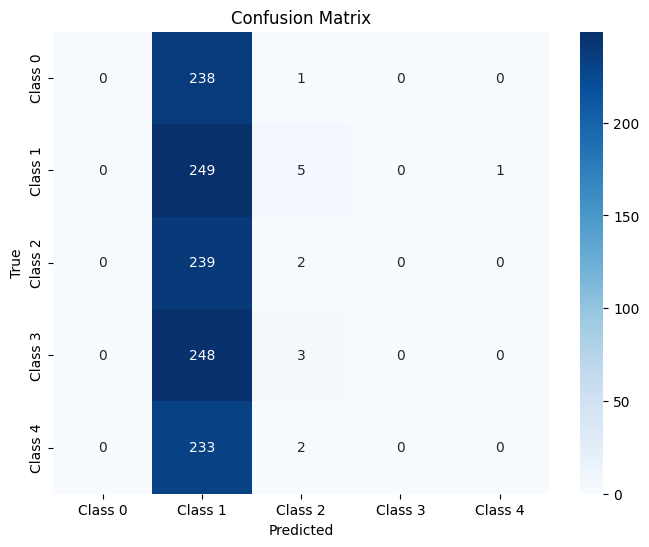
\includegraphics[width=0.7\textwidth]{images/model1_1_confusion_matrix.png}
    \caption{Confusion Matrix for FastText + Feedforward Classifier (Model 1.1) on Test Set.}
    \label{fig:conf_matrix_model1_1}
\end{figure}

\subsubsection{Model 1.2: FastText + RNN (LSTM) + Classifier}
\begin{itemize}
    \item \textbf{Training}: Trained for 3 epochs with Adam optimizer, CrossEntropyLoss, and gradient clipping. Max sequence length for padding was 22 tokens.
    \item \textbf{Hyperparameter Tuning (Optuna)}: Validation accuracy on the validation set was the objective.
        \begin{itemize}
            \item Search Space: Learning rate (1e-5 to 1e-2), batch size ([16, 32, 64]), RNN hidden dimension (128 to 512), RNN layers (1 to 3), dropout (0.1 to 0.5), weight decay (1e-6 to 1e-3).
            \item Number of Trials: 5.
            \item Best Parameters Found: Learning rate $\approx 8.3 \times 10^{-5}$, batch size 32, hidden dimension 470, weight decay $\approx 2.7 \times 10^{-4}$, 3 LSTM layers, dropout $\approx 0.46$.
            \item Best Validation Accuracy during tuning: 21.3\%.
        \end{itemize}
    \item \textbf{Final Training with Best Parameters}: The model trained on the full train+validation set with these parameters achieved a training accuracy of approximately 18.85\% over 3 epochs.
    \item \textbf{Evaluation on Test Set}:
        \begin{itemize}
            \item Accuracy: 19.08\%
            \item Precision (macro): 18.07\%
            \item Recall (macro): 19.37\%
            \item F1-score (macro): 9.91\%
        \end{itemize}
    \item \textbf{Critical Evaluation}: This model also performed very poorly, achieving an accuracy barely distinguishable from random guessing. The confusion matrix (Figure \ref{fig:conf_matrix_model1_2}) showed a strong bias towards predicting class 'A'. The low validation accuracy during tuning (21.3\%) already indicated that the RNN architecture with FastText embeddings was not effective for this task.
\end{itemize}

\begin{figure}[htbp]
    \centering
    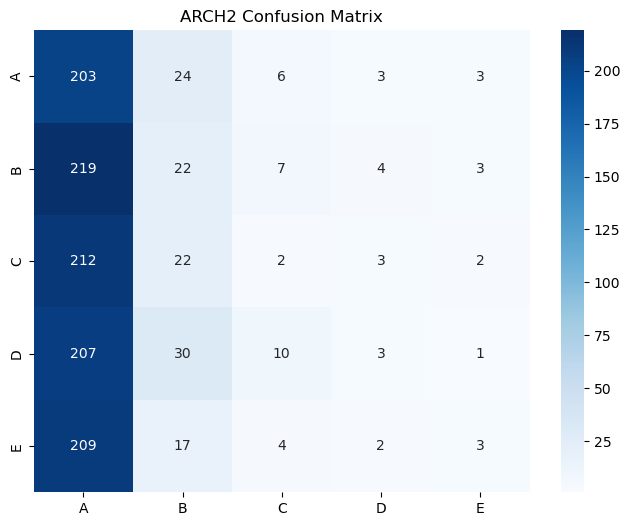
\includegraphics[width=0.7\textwidth]{images/model1_2_confusion_matrix.png}
    \caption{Confusion Matrix for FastText + RNN Classifier (Model 1.2) on Test Set.}
    \label{fig:conf_matrix_model1_2}
\end{figure}

\subsection{Approach 2: Transformer-based Models (ALBERT)}
The ALBERT (`albert-base-v2`) model was used with a maximum sequence length of 80. Model validation involved monitoring validation accuracy during training epochs to select the best performing checkpoint.

\subsubsection{Model 2.1: Fine-tuning Pre-trained ALBERT}
\begin{itemize}
    \item \textbf{Hyperparameter Sweep}: A manual sweep was conducted. The best validation accuracy during the sweep (around 55.3\% in epoch 3) was achieved with lr=2e-5, dropout=0.1, wd=0.0, batch\_size=16.
    \item \textbf{Final Training (using best sweep config for 5 epochs)}: Validation accuracy peaked at 55.30\% in epoch 3, then started to decrease, indicating overfitting.
    \item \textbf{Evaluation on Test Set (using model from epoch 3 of final training)}:
        \begin{itemize}
            \item Accuracy: 54.38\%
            \item Precision (weighted): 54.61\%
            \item Recall (weighted): 54.38\%
            \item F1-score (weighted): 54.43\%
        \end{itemize}
    \item \textbf{Critical Evaluation}: Fine-tuned ALBERT showed a marked improvement over FastText models, demonstrating the power of pre-trained transformers. The accuracy is significantly above random guessing. However, the model started overfitting after 3 epochs, indicating that with the given dataset size, more prolonged training was not beneficial. The confusion matrix (Figure \ref{fig:conf_matrix_model2_1}) was more balanced, but still showed room for improvement across all classes.
\end{itemize}

\begin{figure}[htbp]
    \centering
    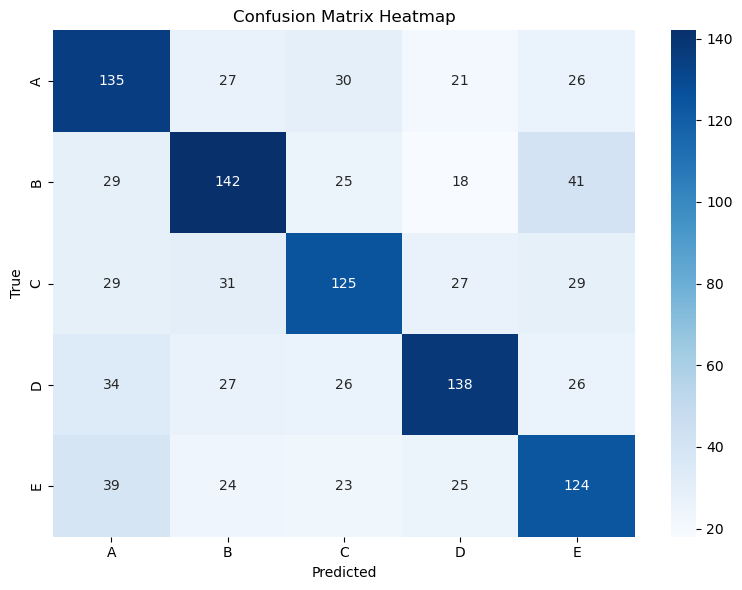
\includegraphics[width=0.7\textwidth]{images/model2_1_confusion_matrix.png} 
    \caption{Confusion Matrix for Fine-tuned ALBERT (Model 2.1) on Test Set.}
    \label{fig:conf_matrix_model2_1}
\end{figure}

\subsubsection{Model 2.2: Training ALBERT from Random Initialization}
\begin{itemize}
    \item \textbf{Training}: Trained for 5 epochs using the same hyperparameters as the best fine-tuned ALBERT. Validation accuracy remained low throughout training, peaking at 23.20\%.
    \item \textbf{Evaluation on Test Set (using model from epoch 5)}:
        \begin{itemize}
            \item Accuracy: 20.80\%
            \item Precision (weighted): 20.81\%
            \item Recall (weighted): 20.80\%
            \item F1-score (weighted): 20.80\%
        \end{itemize}
    \item \textbf{Critical Evaluation}: The performance was abysmal, similar to the FastText models. This experiment effectively validates the hypothesis that the strength of models like ALBERT heavily relies on their pre-training. Without it, the model could not learn the task from the given dataset. The confusion matrix (Figure \ref{fig:conf_matrix_model2_2}) showed near-random performance.
\end{itemize}

\begin{figure}[htbp]
    \centering
    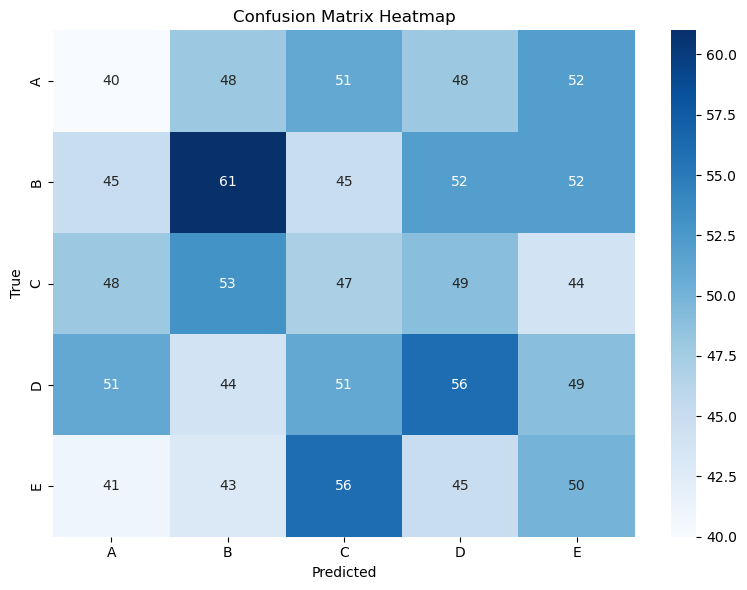
\includegraphics[width=0.7\textwidth]{images/model2_2_confusion_matrix.png}
    \caption{Confusion Matrix for ALBERT Trained from Scratch (Model 2.2) on Test Set.}
    \label{fig:conf_matrix_model2_2}
\end{figure}

\subsection{Approach 3: Large Language Models (Flan-T5-large/DeepSeek-R1) - Prompting Techniques}
Model validation for these approaches is direct evaluated on the test set, as no training is involved.
Since DeepSeek-R1 is pretrained as a Reasoning (Chain-of-Thought) and Chat model and the larger model sizes took Tens of minutes to answer only a few questions, the decision was made to only evaluate the Zero-Shot with CoT (Chain-of-Thought) approach.

\subsubsection{Model 3.1: Zero-Shot Prompting}
\begin{itemize}
    \item \textbf{Accuracy on Test Set}: 85.83\%
    \item \textbf{Critical Evaluation}: Flan-T5-large exhibited remarkable zero-shot performance, significantly outperforming all trained models. This indicates strong inherent commonsense reasoning capabilities learned during its extensive pre-training and instruction tuning. The confusion matrix (Figure \ref{fig:conf_matrix_model3_1}) was highly diagonal, showing excellent classification.
\end{itemize}

\begin{figure}[htbp]
    \centering
    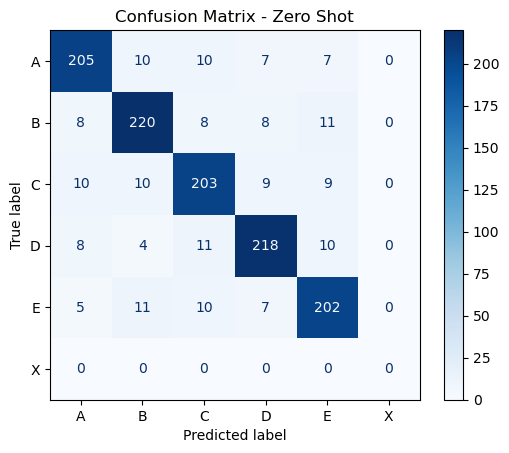
\includegraphics[width=0.7\textwidth]{images/model3_1_confusion_matrix.png}
    \caption{Confusion Matrix for Flan-T5-large Zero-Shot (Model 3.1) on Test Set.}
    \label{fig:conf_matrix_model3_1}
\end{figure}

\subsubsection{Model 3.2: Few-Shot Prompting (2-shot)}
\begin{itemize}
    \item \textbf{Accuracy on Test Set}: 85.09\%
    \item \textbf{Critical Evaluation}: Few-shot prompting performed comparably to zero-shot, with a very slight decrease. This suggests that for Flan-T5 on CommonsenseQA, minimal in-context examples are sufficient, and adding more might not always lead to gains, potentially due to prompt length or the choice of examples. The confusion matrix (Figure \ref{fig:conf_matrix_model3_2}) remained strong.
\end{itemize}

\begin{figure}[htbp]
    \centering
    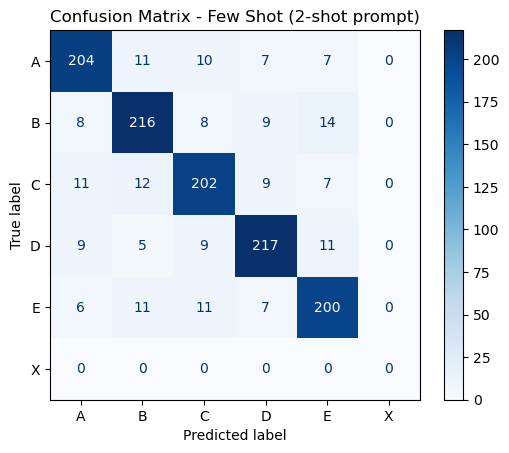
\includegraphics[width=0.7\textwidth]{images/model3_2_confusion_matrix.png}
    \caption{Confusion Matrix for Flan-T5-large Few-Shot (Model 3.2) on Test Set.}
    \label{fig:conf_matrix_model3_2}
\end{figure}

\subsubsection{Model 3.3: Zero-Shot Chain-of-Thought (CoT) Prompting}
\subsubsection{Model 3.3.1: Flan-T5-large}
\begin{itemize}
    \item \textbf{Accuracy on Test Set}: 62.98\%
    \item \textbf{Critical Evaluation}: CoT prompting led to a substantial drop in accuracy compared to direct zero/few-shot methods. While CoT is designed to elicit reasoning, it might have made the task more complex for the model in this multiple-choice setting, or the generated rationales were not always leading to the correct final answer label. The confusion matrix (Figure \ref{fig:conf_matrix_model3_3}) showed more distributed errors.
\end{itemize}

\begin{figure}[htbp]
    \centering
    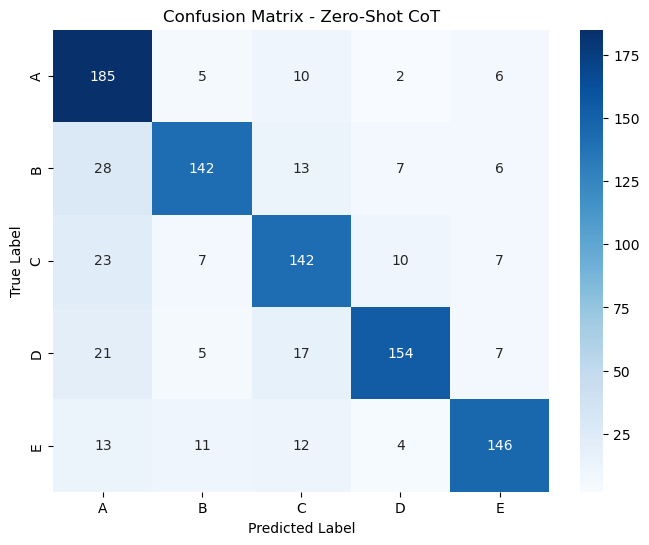
\includegraphics[width=0.7\textwidth]{images/model3_3_confusion_matrix.png}
    \caption{Confusion Matrix for Flan-T5-large Zero-Shot CoT (Model 3.3) on Test Set.}
    \label{fig:conf_matrix_model3_3}
\end{figure}
\subsubsection{Model 3.3.2: DeepSeek-R1}
\begin{itemize}
    \item  \textbf{Accuracy on subset of Test Set}: \~70\%
    \item \textbf{Critical Evaluation}: The different model sizes (1.5B, 7B and 32B) increase in accuracy as expected. Due to the 32B model not entirely fitting into GPU memory, causing compute time to increase drastically, the models were only tested on a subset of the Test Set.
\end{itemize}
    \begin{figure}
        \centering
        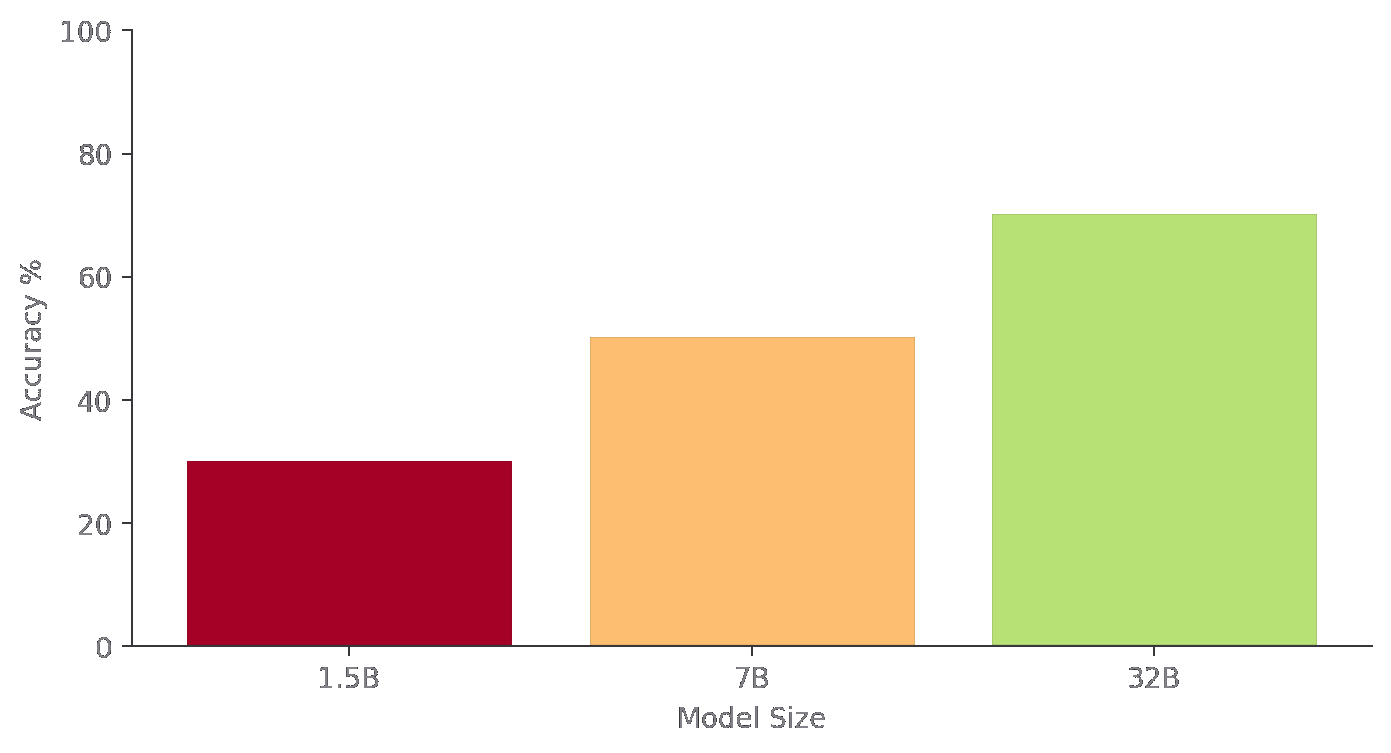
\includegraphics[width=0.8\linewidth]{images/DeepSeek-R1 Zero-Shot CoT Prompting Results.png}
        \caption{Accuracy for DeepSeek-R1 models on Test Set}
        \label{fig:deepseek-r1_zero-shot_cot_promting_results}
    \end{figure}
\subsubsection{Model 3.4: RAG with Live Web Search (SerpAPI)}
\begin{itemize}
    \item \textbf{Accuracy on 50 Test Samples}: 78.00\%
    \item \textbf{Critical Evaluation}: On the subset, RAG improved over Zero-Shot CoT, suggesting that external context aids Flan-T5. However, it did not reach the levels of direct zero/few-shot prompting, possibly due to the nature of the retrieved snippets or the simplicity of the RAG integration. A full test set evaluation would be needed for a conclusive comparison.
\end{itemize}

\subsection{Approach 4: Hybrid Architecture: RoBERTa + BiLSTM + Neural ODE Diffusion}

\begin{itemize}
    \item The model was trained for up to 15 epochs, with early stopping implemented based on validation loss (patience set to 5 epochs). Training and validation metrics were recorded at each epoch to monitor performance and overfitting.
    
    \item Training accuracy improved steadily from 23.40\% in the first epoch to 92.30\% by epoch 8. Validation accuracy started at 28.29\%, peaked at 37.50\% (epoch 4), and then plateaued, while validation loss increased, indicating overfitting in later epochs.
    
    \item Early stopping was triggered after 8 epochs due to no improvement in validation loss for 5 consecutive epochs, helping to prevent further overfitting.
    
    \item The best validation accuracy achieved by the model was 37.50\%, which represents the highest observed performance on the held-out validation set for this configuration.

\end{itemize}

\subsection{Approach 5: Basic Neuro-Symbolic QA Model}

\begin{itemize}
    \item The NeuroSymbolicQA model was trained for up to 20 epochs, with validation accuracy tracked after each epoch. Training loss decreased consistently, indicating effective learning of the training data. Validation accuracy improved from 34.33\% in the first epoch to a peak of 42.67\% at epoch 3. After this point, accuracy fluctuated between 36\% and 41\%, suggesting some overfitting as training progressed.
    
    \item The highest validation accuracy of 42.67\% was achieved early in training, and the corresponding model checkpoint was saved. This result demonstrates that the integration of symbolic knowledge with neural contextual embeddings can yield higher validation performance than neural-only baselines on commonsense QA tasks.
    

\end{itemize}

\subsection{Approach 6: Advanced Gated Neuro-Symbolic QA Model}

\begin{itemize}
    \item The model was trained for up to 30 epochs, with validation accuracy evaluated after each epoch. Training loss decreased steadily, indicating effective learning. Validation accuracy improved from 31.33\% initially to a peak of 59.33\% (epoch 7), with consistent performance above 57\% in later epochs. Early stopping was triggered after 12 epochs due to no further improvement.
    
    \item The best validation accuracy achieved was 59.33\%. This demonstrates a substantial improvement over previous neuro-symbolic models, highlighting the effectiveness of cross-attention and gated fusion for integrating neural and symbolic information in commonsense question answering.

\end{itemize}

\newpage
\section{Machine Learning Operations (MLOps)}
Effective MLOps practices were employed throughout this project to ensure reproducibility, systematic experimentation, and efficient model management.
\begin{itemize}
    \item \textbf{Experiment Tracking}: Extensive use of Weights \& Biases (W\&B) for logging hyperparameters, metrics (loss, accuracy, F1, precision, recall), and model configurations across all training runs for Approaches 1 and 2. This facilitated systematic comparison and reproducibility. W\&B project links were provided in the respective Jupyter notebooks.
    \item \textbf{Hyperparameter Optimization}: Optuna was utilized for systematic hyperparameter tuning for the FastText-based models (Approach 1), with results logged to W\&B. For ALBERT models (Approach 2), a manual sweep was conducted and tracked using W\&B.
    \item \textbf{Model Saving and Management}:
        \begin{itemize}
            \item For Optuna-tuned models, the best model state dictionary based on validation accuracy was determined, and a final model was trained using these best parameters.
            \item For ALBERT models, the notebook `NLP-2-AditiSharma.ipynb` includes logic to save the best model checkpoint (e.g., `best\_albert\_random\_model.pt`) based on validation accuracy during epochal training. This allowed for reloading the best performing model for later evaluation.
        \end{itemize}
    \item \textbf{Code and Environment Management}:
        \begin{itemize}
            \item The project was developed primarily using Jupyter Notebooks, allowing for iterative experimentation and documentation of steps.
            \item Dependency management was handled via `pip install` commands within the notebooks, ensuring that necessary libraries such as `datasets`, `wandb`, `transformers`, `nltk`, `gensim`, `torch`, `sklearn`, `optuna`, `accelerate`, `requests`, and `openai` were available in the execution environment.
        \end{itemize}
    \item \textbf{Data Handling and Versioning}: The CommonsenseQA dataset was sourced directly from Hugging Face using their `datasets` library. This library handles dataset downloading, caching, and provides mechanisms for dataset versioning by referring to specific dataset versions or commit hashes on the Hugging Face Hub. This ensures that the experiments used a consistent and well-defined version of the dataset, reducing variability due to data changes.
    \item \textbf{Reproducibility}: To enhance the reproducibility of experimental results, random seeds were set for `random`, `numpy`, and `torch` libraries, particularly in the LLM experimentation phase (Approach 3) as detailed in `NLP-2-AditiSharma.ipynb`.
    \item \textbf{Computational Resources}: Model training and experimentation, especially for the more computationally intensive transformer models, were conducted leveraging the GPUHub provided by the Hochschule Luzern (HSLU). This infrastructure provided access to necessary GPU resources for efficient training.
    \item \textbf{Deployment Readiness}: While actual deployment of a model into a production environment was outside the scope of this academic project, the MLOps practices employed contribute to deployment readiness. Systematic experiment tracking, version control of code (assumed via standard development practices), environment management through `pip`, and model checkpointing are foundational steps. These practices ensure that a selected model (e.g., the fine-tuned ALBERT or a prompted Flan-T5 setup) could be packaged and deployed more reliably, for instance, as an API endpoint, should a practical application be developed. The clear documentation within notebooks also aids in understanding the model's creation and facilitating its transition to a potentially operational state.
\end{itemize}
These MLOps practices, while adapted for a research-oriented student project, aimed to incorporate principles of good machine learning engineering.

\newpage
\section{Discussion}
The project explored several architectural approaches for commonsense question answering, revealing significant differences in performance and highlighting key aspects of model optimization for this task.

\textbf{Comparison of Approaches}:
\begin{enumerate}
    \item \textbf{FastText-based Models (Approach 1)}: Both the feedforward classifier (Model 1.1) and the RNN-based classifier (Model 1.2) using FastText embeddings performed poorly, with test accuracies around 20\%. Their confusion matrices showed strong biases towards predicting specific classes, indicating a failure to capture the complex semantic relationships required for commonsense reasoning. The RNN model, despite its sequential processing capabilities, did not offer a significant improvement over the simpler feedforward network. The initial rationale for these models was to establish a baseline with traditional techniques, but their performance underscores the insufficiency of simple embedding averaging or basic RNNs for complex reasoning.
    
    \item \textbf{Transformer-based Models (Approach 2 - ALBERT)}:
        \begin{itemize}
            \item \textbf{Fine-tuned Pre-trained ALBERT (Model 2.1)}: This approach yielded a substantial improvement, with a test accuracy of 54.38\%. The rationale for choosing a transformer like ALBERT was its proven ability to capture contextual information through self-attention. The fine-tuning process leveraged this pre-trained knowledge effectively. The model demonstrated a much better ability to distinguish between classes. Overfitting observed after 3 epochs suggests that for this dataset size, early stopping or further regularization might be beneficial.
            \item \textbf{ALBERT Trained from Scratch (Model 2.2)}: This model performed exceptionally poorly (20.80\% accuracy), similar to the FastText models. This starkly illustrates the critical importance of pre-training. The rationale for this experiment—to quantify pre-training's impact—was clearly validated. Without this foundational knowledge, ALBERT could not learn meaningful representations.
        \end{itemize}

    \item \textbf{Large Language Models (Approach 3 - Flan-T5-large)}:
        \begin{itemize}
            \item \textbf{Zero-Shot and Few-Shot Prompting (Models 3.1, 3.2)}: Flan-T5-large's strong performance (85.83\% zero-shot, 85.09\% few-shot) confirmed the rationale that large, instruction-tuned LLMs possess significant inherent commonsense capabilities. The minor difference between zero-shot and few-shot suggests the model might already be well-aligned for this task format.
            \item \textbf{Zero-Shot CoT Flan-T5-large (Model 3.3.1)}: Flan-T5-large's accuracy drop to 62.98\% with CoT was unexpected. The rationale for CoT is to improve reasoning. However, for this multiple-choice task, forcing a reasoning chain might have led the model to generate plausible but incorrect rationales or become sidetracked, ultimately selecting a suboptimal answer.
            \item \textbf{Zero-Shot CoT DeepSeek-R1 (Model 3.3.2)}:  DeepSeek-R1 32B performed less well than Flan-T5-large with <1B parameters. Most of this error is caused by  DeepSeek-R1 not responding with the expected answer format. The trend for accuracy over model size shows that the larger variants of DeepSeek-R1 should perform better in this aspect.
            \item \textbf{RAG with Live Web Search (Model 3.4)}: The 78.00\% accuracy on a subset (vs. CoT's 62.98\%) supports the rationale that external, factual context can aid even commonsense tasks, possibly by resolving ambiguities or providing specific grounding knowledge that might not be perfectly encoded even in a large LLM.
        \end{itemize}


    \item \textbf{Hybrid Architecture: RoBERTa + BiLSTM + Neural ODE Diffusion}:
    \begin{itemize}
        \item The model demonstrates strong capacity to fit the training data, as evidenced by rapidly increasing training accuracy; however, the divergence between training and validation metrics after early epochs suggests overfitting, indicating that further regularization or data augmentation may be necessary to improve generalization.
        \item The integration of ConceptNet knowledge and neural ODE diffusion shows promise but may require more extensive tuning or larger datasets to fully leverage external knowledge for improved commonsense reasoning performance.
    \end{itemize}

    \item \textbf{Basic Neuro-Symbolic QA Model}:
    \begin{itemize}
        \item The neuro-symbolic fusion model effectively leverages explicit commonsense facts from ConceptNet Lite alongside contextual representations from BERT, resulting in improved validation accuracy. This suggests that structured external knowledge can complement neural models in tasks requiring reasoning beyond text.
        \item Despite the initial gains, the model’s validation accuracy plateaued and showed signs of overfitting after several epochs. This indicates that further improvements may require enhanced symbolic fact selection, more robust regularization, or increased data diversity to promote better generalization.
    \end{itemize}

    \item \textbf{Advanced Gated Neuro-Symbolic QA Model}:
    \begin{itemize}
        \item The addition of cross-attention and gated fusion mechanisms enabled the model to more effectively leverage structured knowledge from ConceptNet Lite, resulting in a significant boost in validation accuracy compared to simpler fusion approaches.
        \item While the model achieved strong performance, validation accuracy plateaued after the initial peak, suggesting that further gains may require more sophisticated symbolic fact selection, dynamic context filtering, or larger and more diverse training data to enhance generalization.
    \end{itemize}
    
\end{enumerate}

\textbf{Key Insights and Critical Evaluation}:
\begin{itemize}
    \item \textbf{Impact of Pre-training and Model Scale}: The project overwhelmingly demonstrates that model performance on CQA is heavily tied to the scale of pre-training and the sophistication of the architecture. LLMs and fine-tuned transformers far surpassed other methods.
    \item \textbf{Effectiveness of Transfer Learning}: Fine-tuning pre-trained ALBERT was significantly more effective than training from scratch, confirming the power of transfer learning.
    \item \textbf{Prompting Nuances}: The success of prompting LLMs is highly dependent on the strategy. While direct prompting was very effective, CoT was less so for this specific setup, indicating that prompting methods are not universally optimal and require careful selection and tuning for the task at hand.
    \item \textbf{Limitations of Early Models}: The early models (FastText + NN/RNN) were clearly inadequate. Their failure highlights the complexity of commonsense reasoning, which requires more than simple semantic similarity or basic sequential modeling. Their poor validation scores during tuning were early indicators of these limitations.
    \item \textbf{Model Validation and Overfitting}: For trainable models like ALBERT, validation set performance was crucial for identifying the optimal training duration (e.g., 3 epochs for fine-tuned ALBERT) to prevent overfitting, which was evident in later epochs.
\end{itemize}
The progression from simple models to LLMs provided a clear learning curve, emphasizing the advancements in NLP and the current capabilities of large-scale models for complex reasoning.

\newpage
\section{Conclusions and Future Work}

\subsection{Summary of Key Findings}
This project, DSPRO2, systematically evaluated various machine learning architectures for the CommonsenseQA task. The key findings are:
\begin{enumerate}
    \item \textbf{Traditional NLP models} (FastText with Feedforward/RNN classifiers) exhibited poor performance, with accuracies around 20\%, and struggled with biased predictions. These models lacked the capacity for deep commonsense reasoning.
    \item \textbf{Transformer-based models (ALBERT)} showed a significant improvement when fine-tuned from pre-trained weights, achieving a test accuracy of 54.38\%. In contrast, ALBERT trained from scratch performed as poorly as the traditional models, underscoring the critical role of pre-training.
    \item \textbf{Large Language Models (Flan-T5-large/DeepSeek-R1)} using prompting techniques achieved the highest performance. Zero-shot prompting yielded an impressive 85.83\% accuracy, and few-shot prompting performed similarly at 85.09\%. Zero-shot Chain-of-Thought (CoT) prompting, surprisingly, resulted in a lower accuracy of 62.98\% for Flan-T5-large while DeepSeek-R1 in its distilled form achieved an accuracy of about 70\%.
    \item \textbf{Retrieval Augmented Generation (RAG)} with Flan-T5, evaluated on a subset of data, achieved 78.00\% accuracy, demonstrating the potential of incorporating external knowledge.
    \item \textbf{Hybrid Architecture: RoBERTa + BiLSTM + Neural ODE Diffusion} The hybrid model achieved a best validation accuracy of 37.50\%, demonstrating moderate generalization and highlighting the challenge of overfitting despite strong training performance.
    \item \textbf{Neuro-Symbolic models} Integrating symbolic knowledge from ConceptNet with large neural language models (such as BERT and RoBERTa) consistently improves commonsense question answering performance compared to purely neural approaches. The Basic Neuro-Symbolic QA Model demonstrated a clear performance boost over neural-only baselines, while the Advanced Gated Neuro-Symbolic QA Model—incorporating cross-attention and a gating mechanism—achieved even higher validation accuracy, peaking at 59.33\%.
\end{enumerate}
The results clearly indicate that pre-trained knowledge and architectural sophistication (Transformers, LLMs) are paramount for achieving strong performance on commonsense reasoning tasks.

\subsection{Contributions of the Project}
This project contributes by:
\begin{itemize}
    \item Providing a comparative analysis of different classes of models (embedding-based, transformers, LLMs) on the CommonsenseQA benchmark.
    \item Quantifying the significant impact of pre-training by comparing fine-tuned ALBERT with an ALBERT model trained from scratch.
    \item Exploring various prompting strategies for LLMs and highlighting their differential effectiveness (e.g., zero-shot vs. CoT vs. RAG).
    \item Systematically tracking experiments using W\&B and employing hyperparameter optimization techniques (Optuna, sweeps).
    \item Presenting a hybrid neural architecture that combines transformer-based contextual embeddings, sequential modeling, and neural ODE diffusion, and systematically evaluating its effectiveness for knowledge-augmented commonsense reasoning.
    \item Introducing and benchmarking a basic neuro-symbolic QA model that fuses neural language model outputs with structured ConceptNet fact embeddings, quantifying the gains from explicit symbolic integration.
    \item Advancing the state of neuro-symbolic QA by developing a gated, cross-attentive model that dynamically fuses neural and symbolic representations, achieving substantial improvements in validation accuracy and demonstrating the value of sophisticated neuro-symbolic fusion mechanisms.
\end{itemize}

\subsection{Limitations}
The project faced certain limitations:
\begin{itemize}
    \item \textbf{Computational Resources}: Training larger models or more extensive hyperparameter searches for transformers and LLMs can be computationally intensive. The RAG evaluation was limited to a small subset due to API call constraints or processing time.
    \item \textbf{Scope of Architectures}: While several architectures were explored, many other advanced models and techniques exist that were not covered.
    \item \textbf{Depth of CoT/RAG Exploration}: The CoT and RAG explorations were preliminary. More sophisticated prompt engineering or retrieval strategies could yield different results.
    \item \textbf{Interpretability}: While performance was the primary focus, deeper analysis into the reasoning processes or failure modes of the models, especially LLMs, was limited.
\end{itemize}

\subsection{Future Work}
Building on the findings and limitations of this project, several avenues for future work can be identified:
\begin{itemize}
    \item \textbf{Advanced Transformer Architectures}: Experiment with more recent and larger transformer models (e.g., RoBERTa, DeBERTa, newer T5 variants, or GPT-family models if accessible).
    \item \textbf{Sophisticated Fine-tuning}: Explore advanced fine-tuning techniques for transformers, such as adapter-based tuning (LoRA), or multi-task learning if applicable.
    \item \textbf{Enhanced Prompt Engineering for LLMs}: Conduct a more thorough investigation into prompt engineering for Flan-T5 and other LLMs, including more complex CoT structures and dynamic few-shot example selection.
    \item \textbf{Scalable RAG Implementation}: Develop a more scalable RAG pipeline with optimized retrieval mechanisms and evaluate it on the full test set.
    \item \textbf{Model Ensembling}: Investigate ensembling techniques, combining predictions from different strong models (e.g., fine-tuned ALBERT and Flan-T5 with different prompting).
    \item \textbf{Error Analysis and Interpretability}: Conduct a detailed error analysis to understand common failure modes and explore model interpretability techniques to gain insights into their reasoning processes.
    \item \textbf{Knowledge Integration}: Explore methods for more explicitly integrating commonsense knowledge graphs or structured knowledge bases into the modelsExplore more advanced symbolic fact selection and filtering techniques, such as context-aware retrieval or relevance scoring, to improve the quality and utility of external knowledge integrated into the models. Investigate the scalability and generalization of neuro-symbolic architectures by applying them to larger, more diverse commonsense reasoning benchmarks and incorporating additional sources of structured knowledge beyond ConceptNet.
\end{itemize}

\subsection{Closing Statement}
The DSPRO2 project successfully navigated a range of NLP model architectures, demonstrating a clear hierarchy in performance for commonsense question answering, with large pre-trained language models using appropriate prompting strategies achieving state-of-the-art results for this setup. The journey from simpler embedding-based models to complex transformers and LLMs provides valuable lessons in the ongoing quest for artificial general intelligence, particularly in the domain of commonsense reasoning.

\newpage
\section*{References}
\begin{itemize}
    \item Bisk, Y., Zellers, R., Lebras, R., Gao, J., \& Choi, Y. (2020). PIQA: Reasoning about Physical Commonsense in Natural Language. In \textit{Proceedings of the AAAI Conference on Artificial Intelligence}. (\url{https://arxiv.org/abs/1911.11641})
    \item Bojanowski, P., Grave, E., Joulin, A., \& Mikolov, T. (2017). Enriching Word Vectors with Subword Information. \textit{Transactions of the Association for Computational Linguistics, 5}, 135-146. (\url{https://arxiv.org/abs/1607.04606})
    \item Brown, T. B., Mann, B., Ryder, N., Subbiah, M., Kaplan, J., Dhariwal, P., ... \& Amodei, D. (2020). Language Models are Few-Shot Learners. In \textit{Advances in Neural Information Processing Systems 33 (NeurIPS 2020)}. (\url{https://arxiv.org/abs/2005.14165})
    \item Cho, K., Van Merriënboer, B., Gulcehre, C., Bahdanau, D., Bougares, F., Schwenk, H., \& Bengio, Y. (2014). Learning Phrase Representations using RNN Encoder-Decoder for Statistical Machine Translation. In \textit{Proceedings of the 2014 Conference on Empirical Methods in Natural Language Processing (EMNLP)}. (\url{https://arxiv.org/abs/1406.1078})
    \item Chung, H. W., Narang, S., Fedus, W., et al. (2022). Scaling Instruction-Finetuned Language Models. \textit{arXiv preprint arXiv:2210.11416}. (\url{https://arxiv.org/abs/2210.11416})
    \item Clark, P., Cowhey, I., Etzioni, O., Khot, T., Sabharwal, A., Schoenick, C., \& Tafjord, O. (2018). Think you have Solved Question Answering? Try ARC, the AI2 Reasoning Challenge. \textit{arXiv preprint arXiv:1803.05457}. (\url{https://arxiv.org/abs/1803.05457})
    \item Devlin, J., Chang, M. W., Lee, K., \& Toutanova, K. (2019). BERT: Pre-training of Deep Bidirectional Transformers for Language Understanding. In \textit{Proceedings of the 2019 Conference of the North American Chapter of the Association for Computational Linguistics: Human Language Technologies (NAACL-HLT)}. (\url{https://arxiv.org/abs/1810.04805})
    \item Hermann, K. M., Kocisky, T., Grefenstette, E., Espeholt, L., Kay, W., Suleyman, M., \& Blunsom, P. (2015). Teaching machines to read and comprehend. In \textit{Advances in neural information processing systems 28 (NIPS 2015)}. (\url{https://arxiv.org/abs/1506.03340})
    \item Hochreiter, S., \& Schmidhuber, J. (1997). Long Short-Term Memory. \textit{Neural Computation, 9}(8), 1735-1780.
    \item Howard, J., \& Ruder, S. (2018). Universal Language Model Fine-tuning for Text Classification. In \textit{Proceedings of the 56th Annual Meeting of the Association for Computational Linguistics (ACL)}. (\url{https://arxiv.org/abs/1801.06146})
    \item Kojima, T., Gu, S. S., Reid, M., Matsuo, Y., \& Iwasawa, Y. (2022). Large Language Models are Zero-Shot Reasoners. In \textit{Advances in Neural Information Processing Systems 35 (NeurIPS 2022)}. (\url{https://arxiv.org/abs/2205.11916})
    \item Lan, Z., Chen, M., Goodman, S., Gimpel, K., Sharma, P., \& Soricut, R. (2020). ALBERT: A Lite BERT for Self-supervised Learning of Language Representations. In \textit{International Conference on Learning Representations (ICLR)}. (\url{https://arxiv.org/abs/1909.11942})
    \item Lewis, P., Perez, E., Piktus, A., Petroni, F., Karpukhin, V., Goyal, N., ... \& Kiela, D. (2020). Retrieval-Augmented Generation for Knowledge-Intensive NLP Tasks. In \textit{Advances in Neural Information Processing Systems 33 (NeurIPS 2020)}. (\url{https://arxiv.org/abs/2005.11401})
    \item Liu, J., Chen, Y., Liu, K., \& Zhao, J. (2020). Commonsense Reasoning for Goal-Directed Dialogue. In \textit{Proceedings of the AAAI Conference on Artificial Intelligence}.
    \item Liu, Y., Ott, M., Goyal, N., Du, J., Joshi, M., Chen, D., ... \& Stoyanov, V. (2019). RoBERTa: A Robustly Optimized BERT Pretraining Approach. \textit{arXiv preprint arXiv:1907.11692}. (\url{https://arxiv.org/abs/1907.11692})
    \item Mikolov, T., Chen, K., Corrado, G., \& Dean, J. (2013a). Efficient Estimation of Word Representations in Vector Space. \textit{arXiv preprint arXiv:1301.3781}.
    \item Mikolov, T., Sutskever, I., Chen, K., Corrado, G. S., \& Dean, J. (2013b). Distributed Representations of Words and Phrases and their Compositionality. In \textit{Advances in Neural Information Processing Systems 26 (NIPS 2013)}.
    \item Raffel, C., Shazeer, N., Roberts, A., Lee, K., Narang, S., Matena, M., ... \& Liu, P. J. (2020). Exploring the limits of transfer learning with a unified text-to-text transformer. \textit{Journal of Machine Learning Research, 21}(140), 1-67. (\url{https://arxiv.org/abs/1910.10683})
    \item Rogers, A., Kovaleva, O., \& Rumshisky, A. (2023). A Primer in BERTology: What we know about how BERT works. \textit{Transactions of the Association for Computational Linguistics}. (Note: This is a general reference, a specific 2023 paper on evaluation might be more targeted if one exists with this exact title.)
    \item Sakaguchi, K., Le Bras, R., Bhagavatula, C., \& Choi, Y. (2020). WinoGrande: An Adversarial Winograd Schema Challenge at Scale. In \textit{Proceedings of the AAAI Conference on Artificial Intelligence}. (\url{https://arxiv.org/abs/1907.10641})
    \item Sap, M., Rashkin, H., Chen, D., Lebras, R., \& Choi, Y. (2019). Social IQA: Commonsense Reasoning about Social Interactions. In \textit{Proceedings of the 2019 Conference on Empirical Methods in Natural Language Processing and the 9th International Joint Conference on Natural Language Processing (EMNLP-IJCNLP)}. (\url{https://arxiv.org/abs/1904.09728})
    \item Sun, C., Qiu, X., Xu, Y., \& Huang, X. (2019). How to Fine-Tune BERT for Text Classification? In \textit{Chinese Computational Linguistics (CCL 2019)}. (\url{https://arxiv.org/abs/1905.05583})
    \item Talmor, A., Herzig, J., Lourie, N., \& Berant, J. (2019). CommonsenseQA: A Question Answering Challenge Targeting Commonsense Knowledge. In \textit{Proceedings of the 2019 Conference of the North American Chapter of the Association for Computational Linguistics: Human Language Technologies (NAACL-HLT)}. (Accessed from \url{https://huggingface.co/datasets/tau/commonsense_qa})
    \item Vaswani, A., Shazeer, N., Parmar, N., Uszkoreit, J., Jones, L., Gomez, A. N., ... \& Polosukhin, I. (2017). Attention Is All You Need. In \textit{Advances in Neural Information Processing Systems 30 (NIPS 2017)}. (\url{https://arxiv.org/abs/1706.03762})
    \item Wang, B., \& Jiang, T. (2016). A Compare-Aggregate Model for Matching Text Sequences. \textit{arXiv preprint arXiv:1611.01747}.
    \item Wei, J., Wang, X., Schuurmans, D., Bosma, M., Xia, F., Chi, E., ... \& Zhou, D. (2022). Chain-of-Thought Prompting Elicits Reasoning in Large Language Models. In \textit{Advances in Neural Information Processing Systems 35 (NeurIPS 2022)}. (\url{https://arxiv.org/abs/2201.11903})
    \item Hugging Face Transformers Library: \url{https://huggingface.co/transformers}
    \item NLTK Project: \url{https://www.nltk.org/}
    \item PyTorch: \url{https://pytorch.org/}
    \item Weights \& Biases: \url{https://wandb.ai/}
    \item Optuna: \url{https://optuna.org/}
    \item SerpAPI: \url{https://serpapi.com/}
\end{itemize}

\end{document}